%begin-include

%In this chapter we present experiments of model selection of cell
% signaling pathways. We divide this chapter in two sections; the first
% section presents experiments to compare two model selection software: 
% ABC-SMC and SigNetMS, both of them presented on
% chapter~\ref{chap:model_selection_methods}. We end the first section
% presenting which software had best fit for our experiments. The
% following section presents experiments of model selection as a feature
% selection problem. We will analyze algorithm trace and what is the
% surface induced by the cost function over the search space.

\section{Choosing a Software for Model Selection}
% To choose a software for model selection we did the same experiment as
% girolami
%
% A simple instance of the model selection problem
% -> the correct model is...
% -> then we create other three models
%   - a simplification
%   - an overly complex model
%   - and an incorrect model
% -> the expected result for this experiment is that the correct model
%  has a higher (possibly be the first), and that the incorrect model
%  should be considered the worst. It is also important to see how the
%  software compares models with similar dynamics and with different
%  levels of complexity.
%  
% Results produced by SigNetMS and ABC-SysBio
% -> we proceeded to run both softwares 
% -> compare the ranking of both software
% -> show how the curve fits on both software
% -> show that there is some parameter value convergence on SigNetMS

To choose between SigNetMS and ABC-SysBio, we performed a model
selection experiment. This experiment, originally performed on the work
of Vyshemirsky and Girolami~\cite{Vyshemirsky2007}, consists in creating
artificial experimental data from a model of cell signaling pathway, and 
then selecting between four different models, including the correct one.
Using SigNetMS and ABC-SysBio we should be able to create a ranking of
the four models, in which we expect to see as the best, the model we
used to create the experimental data. More than that, we should analyze
the produced results to check if simpler models are preferred over
complex models; we should also check if the simulations produced by the
models, with the estimated sample of the posterior distribution of
parameters, approximates experimental data.

\subsection{A simple instance of the model selection problem}
\begin{figure}[h]
\begin{center}
    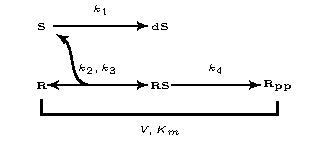
\includegraphics[width=.75\textwidth]{experiments/diagrams/bioinformatics_model1.pdf}
    \caption{A diagram that represents the correct model our simple
model selection experiment. This model represents a common motif, and
has S and Rpp as input and output, respectively. This model contains
five reactions: the decay of S to dS with $k_1$ as reaction rate
constant; the reversible reaction $\ce{S + R <=>[$k_1$][$k_2$] RS}$; the
first order reaction $\ce{RS ->[$k_4$] Rpp}$; and the Michaelis-Menten
reaction $\ce{A ->[$V, K_m$] B}$.}
    \label{fig:experiments:girolami_model1}
    \end{center}
\end{figure}

We start our model selection problem with the correct model, which is 
a signalling pathway composed by five reactions and five chemical 
species. Figure~\ref{fig:experiments:girolami_model1} shows a diagram
with this model. This model represents a common motif, and it has as the 
input signal the chemical species "S", and as the output the chemical 
species "Rpp"; the experimental measurement used is the concentration of 
the output chemical species, which we donote as [Rpp].


In this experiment, for the sake of simplicity, we neglect the units of 
reaction rates constants and initial concentrations. The initial 
concentrations used are:  S $= 1$, R $= 1$, dS $= 0$, RS $= 0$, 
R$_{pp} = 0$. To create the experimental data, the reaction rate 
constants we used have the values: 
$k_1 = 0.07$, $k_2 = 0.6$, $k_3 = 0.05$, $k_4 = 0.3$, $V = 0.017$, and
$K_m = 0.3$. It is important to remember that we discard reaction rate
constant values during model selection; initial concentrations, however,
are still provided during this phase. To generate experimental data, we
simulate the dynamics of this model, using these parameter values, on
the time steps of: 2s, 10s, 20s, 40s, 60s and 100s. Three simulations
are created, and to each one of them we add, for each time measurement,
a Gaussian error with mean $0$ and standard deviation $0.01$. A
representation of the three experiment repetitions are showed on 
figure~\ref{fig:experiments:girolami_simulations}.

% TODO: determine the prior distribution used

% insert simulated data here
\begin{figure}
\begin{center}
    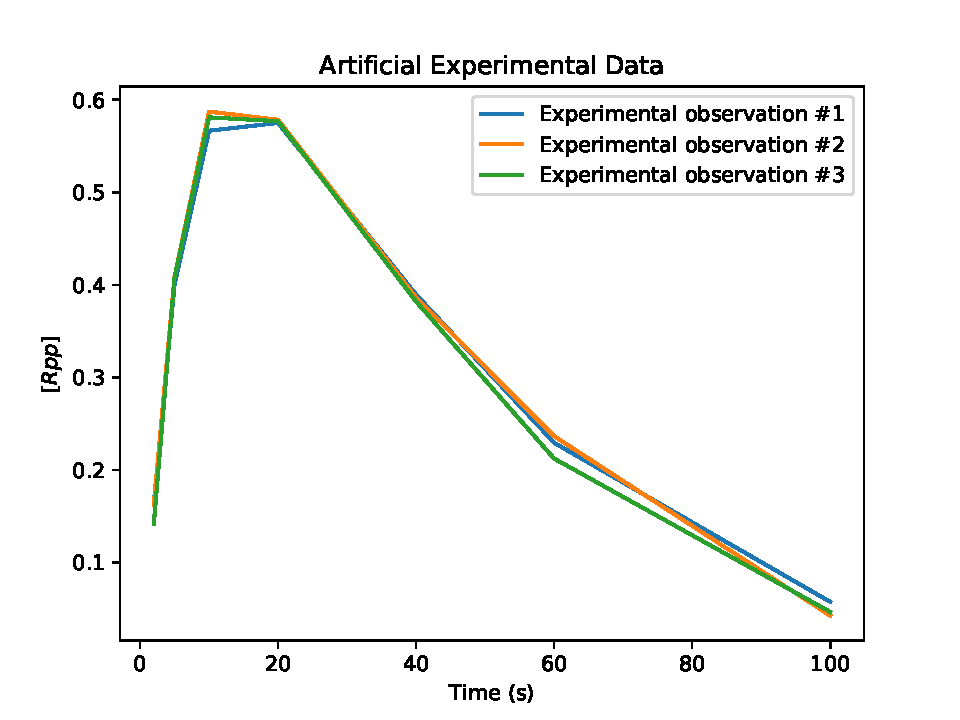
\includegraphics[width=.75\textwidth]{experiments/simulations/girolami_experimental_data.pdf}
    \caption{The dynamics produced by the correct model, with
pre-defined reaction rate constants plus a small Gaussian error, for
each time point. The measurement taken from the model is the
concentration of the Rpp species, which we denote as [Rpp]. We
linearly interpolate the experimental measure points to produce a
continuous dynamics from 2s to 100s.}
    \label{fig:experiments:girolami_simulations}
    \end{center}
\end{figure}

To assess the ranking produced by each of the model selection software,
we compare the first model with three other models (based on the correct
model): a simplified model; an overly simplified model, which should not 
be able to generate the observed dynamics; and, finally, a 
generalization (more complex) model.
Figure~\ref{fig:experiments:girolami_other_models} shows diagrams that
represent the three alternative models.

\begin{figure}[h]
    \centering
    \begin{tabular}{c c}
    \subfigure[simplified model]{
    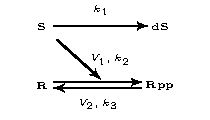
\includegraphics[clip=true,width=.45\linewidth]{experiments/diagrams/bioinformatics_model2.pdf}
    \label{fig:girolami_model2}}
    &
    \subfigure[overly simplified model]{
    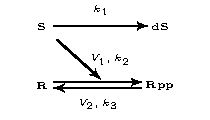
\includegraphics[clip=true,width=.45\linewidth]{experiments/diagrams/bioinformatics_model3.pdf}
    \label{fig:girolami_model3}} 
    \\
\multicolumn{2}{c}{    
    \subfigure[generalization model]{
    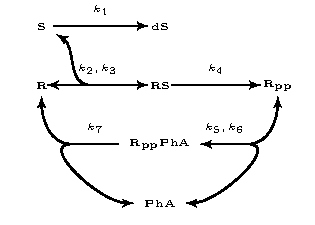
\includegraphics[clip=true,width=.45\linewidth]{experiments/diagrams/bioinformatics_model4.pdf}
    \label{fig:girolami_model4}}
} 
    \end{tabular}
    \caption{The diagrams of three other candidate models, based on the 
correct model that was presented before on 
Figure~\ref{fig:experiments:girolami_model1}. The 
model~\ref{fig:girolami_model2} is a simplification where we neglect the
chemical species RS, and we use the Michaelis-Menten to represent the
reaction $\ce{R -> Rpp}$ with S working as a catalyst.
Model~\ref{fig:girolami_model3} is the over simplified model, as it
neglects the decay of S; we do not expect this model to reproduce
experimental data, since the constant concentration level of S tend to
continuously produce Rpp, a species that, after 20 seconds, has a
monotonic decreasing concentration. Finally,
Model~\ref{fig:girolami_model4} is a generalization of the correct
model, as it generalizes the reaction $\ce{Rpp -> R}$, as instead of 
using the Michaelis-Menten kinetics, we use the enzymatic reaction 
$\ce{Rpp + PhA <=> RppPhA -> R + PhA}$; even though we expect this model
to be able to reproduce observed dynamics, we also expect that the
complexity of this model gets penalized.
}
    \label{fig:experiments:girolami_other_models}
\end{figure}

% -> the expected result for this experiment is that the correct model
%  has a higher (possibly be the first), and that the incorrect model
%  should be considered the worst. It is also important to see how the
%  software compares models with similar dynamics and with different
%  levels of complexity.

Before talking about results produced by different software, we should
note that this choice of candidate models are made so we can analyze
more than the ability of the software to correctly rank the correct
model as the best model. First, consider that we introduced a spurious
model, represented on figure~\ref{fig:girolami_model3} which neglects a
crucial reaction, making it impossible to reproduce the experimental
data; we expect this model to be ranked last between all models. Then,
there are two options to the correct model, one a simplification, and
the other a generalization. For these models, we expect that the
experimental dynamics are possible, however, we should be observant of
how they are ranked according to their complexity. We should remember
that, one of the goals of using a Bayesian approach for model selection
is that these approaches tend to automatically penalize overly complex
models.

% Comparing results of ABC-SMC and SigNetMS
\subsection{Solving a simple model selection instance using ABC-SysBio
and SigNetMS}
% What is the experiment
% What data the experiment produces;
% What are algorithm parameters we used;
% 1 - marginal likelihood of each model
% 2 - a sample of the posterior

% the input and output
After definig the candidate models and producing the artificial
experimental data, we proceeded to perform the experiment of model
selection. The instance related information provided to SigNetMS and 
ABC-SysBio is the same: a model, with predefined initial concentrations
of chemical species; a set of experiments, with the same time steps, 
with measurements of the concentration of Rpp; and a file containing
prior distributions for each one of the model parameters. It is
important to remember that the output produced by each software is
different. SigNetMS produces an estimative of $p({\bm D} | M)$ and also
a sample of the posterior distribution of parameters $p({\bm \theta} |
M, {\bm D})$ which is, in fact, composed by samples of all power
posterior distributions $p_{\beta}({\bm \theta})$ with values as we
described
on~\ref{sec:creating_an_estimative_of_the_marginal_likelihood}.
ABC-SysBio, on the other hand, produces an estimatives of $p({\bm
\theta}, M | {\bm D})$ that might be closer to this target distribution
on each iteration. Note that in this experiment, we need to run SigNetMS
for every model, while on ABC-SysBio we only need to run the software
once for all four candidate models.
% what are algorithm parameter values used

For ABC-SysBio we decided to use its feature of automatically choosing
the schedule of threshold values, which is based on the acceptance of
produced individuals on each iteration. For SigNetMS, we used the
following parameters values: 15000 iterations of the naive burn-in, and
5000 iterations of the posterior shaped burn-in, with 1000 iterations
between covariation matrix rescales, and 3000 iterations of the
Populational MCMC. We used an empiric approach to determine these
parameter values, observing similar results when the number of
iterations are greater then these.

\subsubsection{The ranking produced by ABC-SysBio and SigNetMS}
The ABC-SysBio run created 26 populations of parameter values, each of 
them with 100 individual parameters values. At the last iteration, the 
algorithm stopped with $\epsilon = 1$ and the following estimates: 
\begin{itemize}
    \item{$\hat{p} (M = \text{Correct Model} | {\bm D}, \epsilon = 1) =
        0.005$;}
    \item{$\hat{p} (M = \text{Simplified Model} | {\bm D}, \epsilon = 1)
        = 0.014$;} 
    \item{$\hat{p} (M = \text{Incorrect Model} | {\bm D}, \epsilon = 1)
        = 0.976$;}
    \item{$\hat{p} (M = \text{Generalization Model} | {\bm D}, \epsilon
        = 1) = 0.003$.}
\end{itemize}
These estimates induces the ranking 3, 2, 1, 4.

After running the SigNetMS software four times, one for each model, we
were able to get the following estimates:
\begin{itemize}
    \item{$\log \hat{p}({\bm D} | M = \text{Correct Model}) = 26$}
    \item{$\log \hat{p}({\bm D} | M = \text{Simplified Model}) = 21$}
    \item{$\log \hat{p}({\bm D} | M = \text{Incorrect Model}) = -1$}
    \item{$\log \hat{p}({\bm D} | M = \text{Generalization Model}) =
        19$}
\end{itemize}

% subsubsection Comparing the produced ranking
\subsubsection{Comparing the ranking produced by ABC-SysBio and SigNetMS}
Before comparing the model ranking produced by ABC-SysBio and SigNetMS,
we should state that the ranking achieved by Vyshemirsky and 
Girolami~\cite{Vyshemirsky2007}, on the original work that introduced
this instance, is: Correct Model $\prec$ Generalization Model $\prec$
Simplified Model $\prec$ Incorrect Model. On this work, a methodology
similar to SigNetMS was used.

On ABC-SysBio results, we see that the Correct Model was not ranked
first, and, surprisingly, the Incorrect Model was ranked first. More
than that, when the algorithm stopped, other candidate models were
considered with low probability of being the ``true'' model, and
therefore we cannot strongly state a ranking between the other three
candidates.

On SigNetMS results, we see that the Correct Model was ranked first and 
the Incorrect Model is ranked last as expected. For these two models,
SigNetMS results are equal to the results of Girolami and Vyshemirsky,
and for the other two models, the ranking is the opposite. On SigNetMS,
we ranked the Simplified Model as better than the Generalization Model.

% subsubsection Analyzing the distribution of posteriors
\subsubsection{}
% For now, we can say that SigNetMS is a good software and that it might
% match our needs. To get a better understanding of the results and to
% check if the produced ranking is consistent, we analyzed the...
% For ABC-SysBio too...


\section{Model Selection as a Feature Selection Problem}
